\documentclass[a4paper]{article}
\usepackage[warn]{mathtext}
\usepackage[utf8]{inputenc}
\usepackage[T2A]{fontenc}
\usepackage[english,russian]{babel}
\usepackage{indentfirst}
\usepackage{misccorr}
\usepackage{subcaption}
\captionsetup{compatibility=false}
\usepackage{geometry}
\geometry{verbose,a4paper,tmargin=2cm,bmargin=2cm,lmargin=1.5cm,rmargin=1.5cm}
\usepackage{graphicx}
\usepackage{wrapfig}
\usepackage{amsmath}
\usepackage{fancyhdr}
\usepackage{floatflt}
\usepackage{float}
\usepackage{amssymb}
\usepackage{color}
\usepackage{lscape}
\usepackage{hvfloat}
\usepackage{amsfonts}
\usepackage{euscript}
\usepackage{newunicodechar}
\usepackage{booktabs}
\usepackage{epigraph}
\usepackage{csquotes} 
\usepackage{hyperref}

\hypersetup{
    colorlinks=true,      
    urlcolor=blue,
    linkcolor= blue
}

\begin{document}
\newcommand{\apple}{\char"F8FF}



\begin{titlepage}
    \vspace*{4cm}
	\centering
    {\scshape\LARGE Московский физико-технический институт\par}
	\vspace{1cm}
	{\scshape\Large Эсее по защите информации\par}
	\vspace{1cm}
    {\huge\bfseries  Криптографические протоколы. Протокол Girault.\par}
	\vspace{2cm}
	\vfill
\begin{flushright}
	{\large Выполнила студентка Б01-907}\par
	\vspace{0.3cm}
	{\LARGE Юлия Прохорова}
\end{flushright}
	
	\vfill
Долгопрудный, 2022
% Bottom of the page
\end{titlepage}

\pagestyle{fancy} 
\fancyhead[L]{Криптографические протоколы. Протокол Girault.}
\fancyhead[R]{Юля Прохорова, Б01-907}
\fancyhead[C]{}
\fancyfoot[C]{ \noindent\rule{\textwidth}{0.4pt} \thepage }

\tableofcontents

\newpage

\epigraph{Кто владеет информацией, тот владеет и миром.}{Натан Майер Ротшильд}

\section{Введение}
Криптографию называют наукой или даже искусством безопасных сообщений. Криптография встречается и в повседневной жизни, например, можно зашифровать ваш личный дневник, чтобы никто другой не смог его прочитать. Но здесь мы поговорим о криптографии, которая защищает важные файлы, документы или банковские счета от любого, кто попытается их прочесть.
  \par
  \begin{displayquote}
    Брюс Шнайер пишет: "Если я беру письмо, кладу его в сейф где-нибудь в Нью-Йорке, затем велю Вам прочитать это письмо, то это не безопасность. Это непонятно что. С другой стороны,
  если я беру письмо и кладу его в сейф, затем передаю этот сейф Вам вместе с детальным описанием, передаю также сотню подобных сейфов
  с их комбинациями, чтобы Вы и лучшие "медвежатники мира" могли изучить систему замков, а вы все равно не сможете открыть сейф 
  и прочитать письмо - вот это и есть безопасноть." 
 \end{displayquote}
 
 Современная криптография - общирная область знаний, сложившаяся в результате серьезных исследований на протяжении последних десятков лет. 
 Данная работа направлена на то,
  чтобы познакомить читателя с криптографическими протоколами, а именно с протоколом Girault. Но не обо всем сразу. Начнем с сновных понятий и терминов.

\section{Общая теория}

Обычная ситуация, которую рассматривают, когда изучают криптографию:
\begin{itemize}
    \item есть две стороны: отправитель и получатель;
    \item первый хочет послать сообщение второму;
    \item при этом отправлять сообщение необходимо безопасным образом -  чтобы любой перехвативший не cмог его прочесть.
\end{itemize}
\par В данном случае само сообщение будет называться \textbf{открытым текстом}. Изменение сообщения так, чтобы не была понятна его суть - это \textbf{шифрование}, полученный текст - \textbf{шифротекст}.
\textbf{Дешифрованием} же называется процесс преобразования шифротекста в открытый текст. \textbf{Шифр} представляет собой обратимую математическую функцию, используемая для шифрования и дешифрования.
 
\par Шифрование разделяют на две основные группы: \textbf{симметричные} и соответственно \textbf{ассиметричные}. Для обеих групп необходимо наличия ключа для шифрования и дешифрования, однако в разных группах реализация отличается. В случае симметричных шифров есть два варианта: 
\begin{itemize}
    \item обе операции используют один и тот же ключ $K$;
    \item ключ дешифрования $K_2$ можно получить из ключа шифрования $K_1$ простейшей операцией;
\end{itemize}
Группу симметричных шифров разделяют на:
\begin{itemize}
    \item \textbf{блочные} 
    \begin{itemize}
        \item за одну операцию шифрования происходит преобразование одного блока данных;
        \item размеры блоков одинаковы;
        \item результат шифрования блока может зависеть от предыдущего;
    \end{itemize}
    \item \textbf{потоковые} 
    \begin{itemize}
        \item работают с каждым символом открытого текста по-отдельности;
        \end{itemize}
\end{itemize}
Вернемся к ассиметричным шифрам. Как читатель, вероятно, уже догадался  - для таких шифров ключ для дешифрования $K_2$ получить из ключа шифрования $K_1$ сложно. 
\subsection{Протоколы}
\textbf{Протокол} - порядок действий, предпринемаемых сторонами, чтобы решить поставленную задачу. Каждое действие должно выполняться в свою очередь и только
после окончания предыдущего.
\par
Каждый протокол должен обладать следующими характеристиками:
\begin{itemize}
    \item \textbf{Известность} - каждый участник протокола должен знать протокол и последовательность составляющих его действий;
    \item \textbf{Cогласованность} - каждый участник протокола должен согласиться следовать ему;
    \item \textbf{Отсутствие противоречий (прозрачность)} - каждое действие должно быть определено так, чтобы не было возможности непонимания;
    \item \textbf{Полнота} -  каждой ситуации соответствует определенное заранее действие.
\end{itemize}

Используя криптографический протокол, участники протокола могут:
\begin{itemize}
    \item безопасно передавать друг другу сообщения;
    \item делиться секретом друг с другом;
    \item случайно генерировать случайную последовательность;
    \item подтверждать свою подлинность;
    \item подписывать контракт одновременно.
\end{itemize}

Для демонстрации работы протоколов обычно определяют участников: Alice - начинает протокол, Bob - отвечает, также при необходимости дополнительных сторон появляются Carol и Dave.
\par 
Далее рассмотрим основные виды протоколов: \par
\subsubsection{Протокол с посредником}
\textbf{Посредник} - незаинтересованная 3я сторона, которая завершает протокол. Такой протокол используют, если стороны недоверяют друг другу. При этом все участники протокола принимают за истину все, что скажет посредник. 
Все его действия - правильные, и все стороны протокола уверены в том, что посредник выполнит свою часть протокола.

У данного протокола, как и любого другого существуют недостатки:
\begin{itemize}
    \item сложно доверять безликому посреднику;
    \item компьютерная сеть должна обеспечить поддержку посредника;
    \item возможно возникновение задержек;
    \item посредник должен принимать участие в каждой транзакции, являясь узким местом в реализации протокола;
    \item при попытке взлома сети - посредник слабое звено, так как каждый участник протокола должен доверять ему.
\end{itemize}
\subsubsection{Арбитражные протоколы}
Арбитражный протокол делится на два подпротокола:
\begin{itemize}
    \item протокол без посредника - он выполняется, если стороны смогли самостоятельно договориться;
    \item фактически протокол с посредником, которого приглашают в случае разногласия между сторонами (здесь посредника называют арбитром).
\end{itemize} 
\par 
\textbf{Арбитр} - это незаинтересованное лицо, участвующее в протоколе. Арбитру доверяют обе стороны. Его приглашают для проверки честности выполнения протокола между сторонами.
Хороший арбитражный протокол может не только определить факт мошенничества, но также и определить сторону, которой были совершены злодеяния. Такой протокол лишь обнаруживает мошенничество, но не предсказывает и не предотвращает его.
\subsubsection{Самодостаточные протоколы}
Такие протоколы считают лучшими, так как они обеспечивают полную честность сторон. Для такого протокола не требуется участие какого-либо посредника, даже в критические моменты. Протокол построен так, что при попытке одной стороны смошенничать - другая сразу узнает об этом, а протокол прекратит выполняться.
Однако надо понмать, что не сущетсвует такого самодостаточного протокола, который подходил бы под все ситуации. 
\subsubsection{Попытки вскрытия протоколов}
Существует много способов взломать протокол. Можно просто подслушивать протокол, пробуя добыть информацию - это \textbf{пассивное вскрытие}, здесь взломщик никак не воздействует на сам протокол.
Такой тип взлома относится к взлому с использованием шифротекста. Его сложно обнаружить, поэтому протоколы реализованы таким образом, чтобы предотвратить вскрытие.
Другой способ - \textbf{активное вскрытие }, по сути - просто изменение протокола. Например, можно попробовать подменить сообщение, повторное оправить старое или внести новое.
\par
Пассивные взломщики занимаются сбором информации и криптоанализом сообщений. Активные взломщики стараются получить доступ к ресурсам или ухудшить работу системы.
Взломщиком может оказаться, кто угодно - даже участник протокола. Он может обманывать, выполняя протокол или наоборот не следовать протоколу вовсе. Такой взломщик - мошенник. Пассивные мошенники выполняют правила протокола, но стараются получить больше информации, чем предусмотренно протоколом.
Активные нарушают работу протокола.
\subsection{Распространение ключей}
Для того чтобы создать и настроить надежную сеть необходимо безопасно распределять ключ - так, чтобы два конечных пользователя могли одновременно получить секретный сессионный ключ шифрования. 
\par
Параметры, определяющие качество протокола распространения ключей:
\begin{itemize}
    \item результатом работы протокола является секретный сессионный ключ;
    \item окончание протокола подразумевает под собой успешную взаимную аутентификацию абонентов;
    \item внешний пользователь не должен иметь возможность получить общий сессионный ключ с кем-то из внутренних пользователей;
    \item добавление и удаление участников из сети производится без уведомления всех участников сети.
\end{itemize}
Сети бывают с выделенным доверенным центром и без. Второй вариант плох тем, что с ростом количества участников сети, количество пар мастер-ключей растет с квадратичной скоростью.
\begin{figure}[H]
	\begin{center}
	\begin{minipage}[h]{0.45\linewidth}
	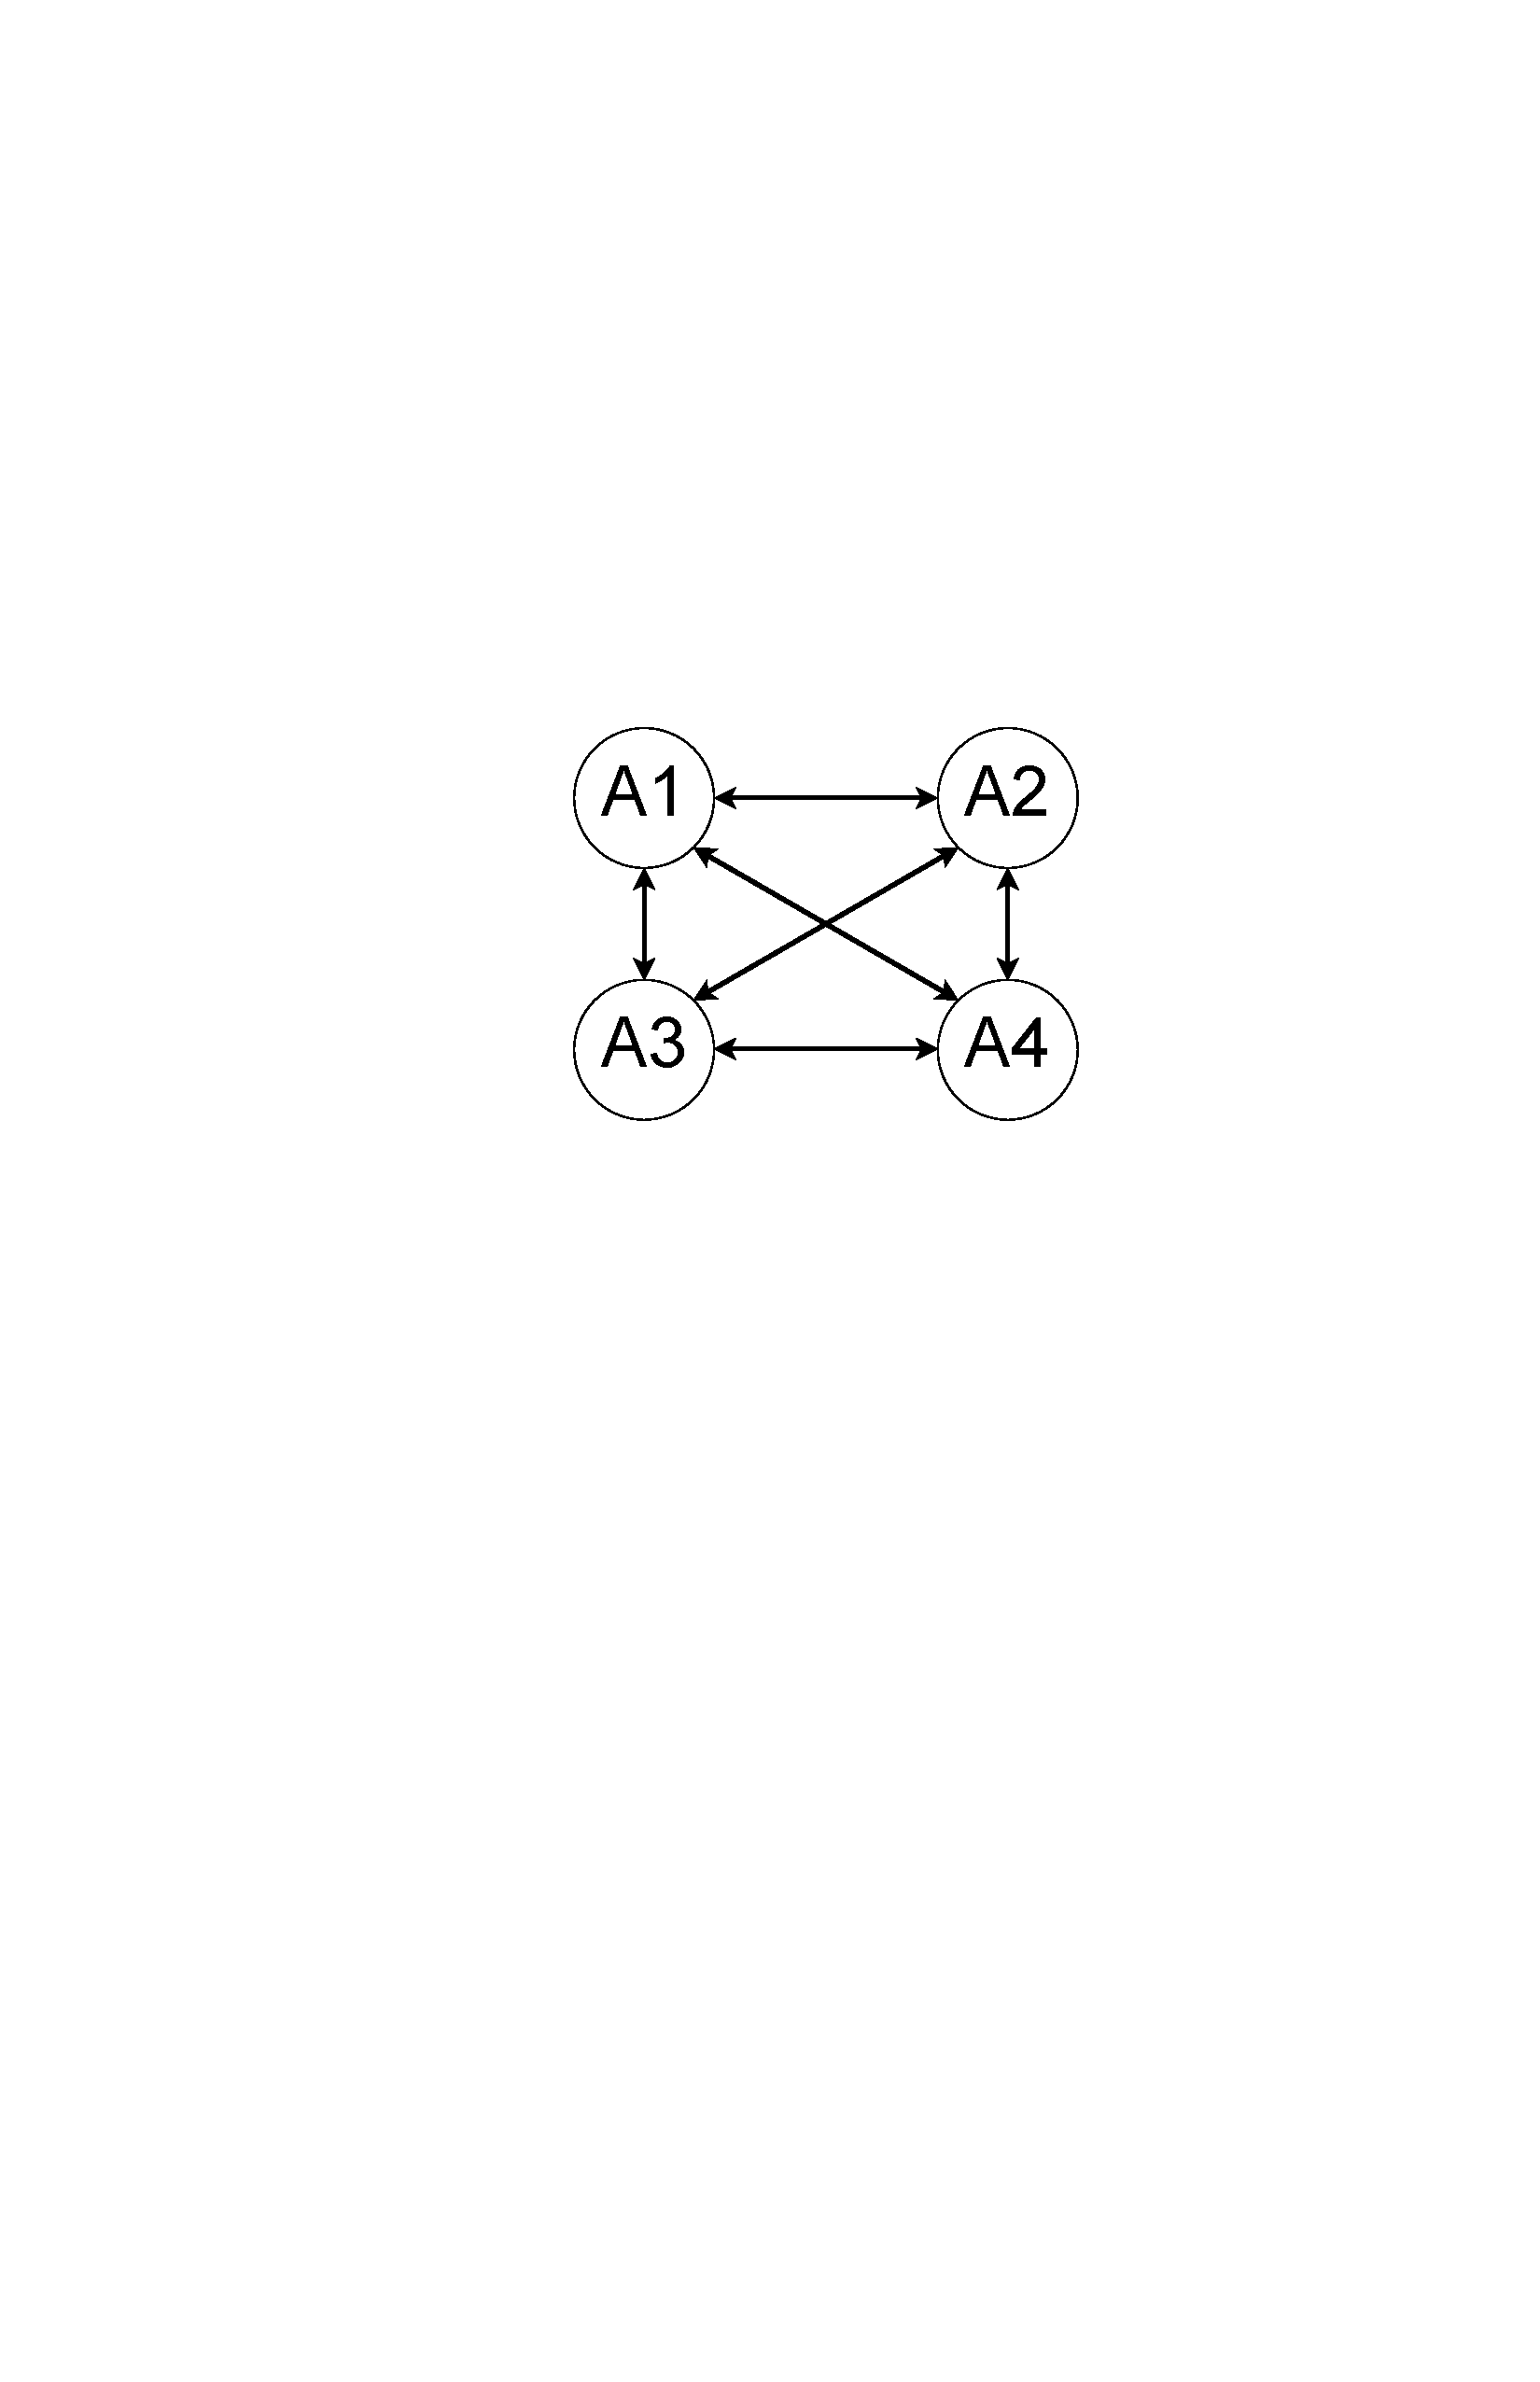
\includegraphics[width=1\linewidth]{pic1.pdf}
	\caption{Сеть без выделенного доверенного центра.} 
    \label{p2}
	\end{minipage}
	\hfill 
	\begin{minipage}[h]{0.43\linewidth}
	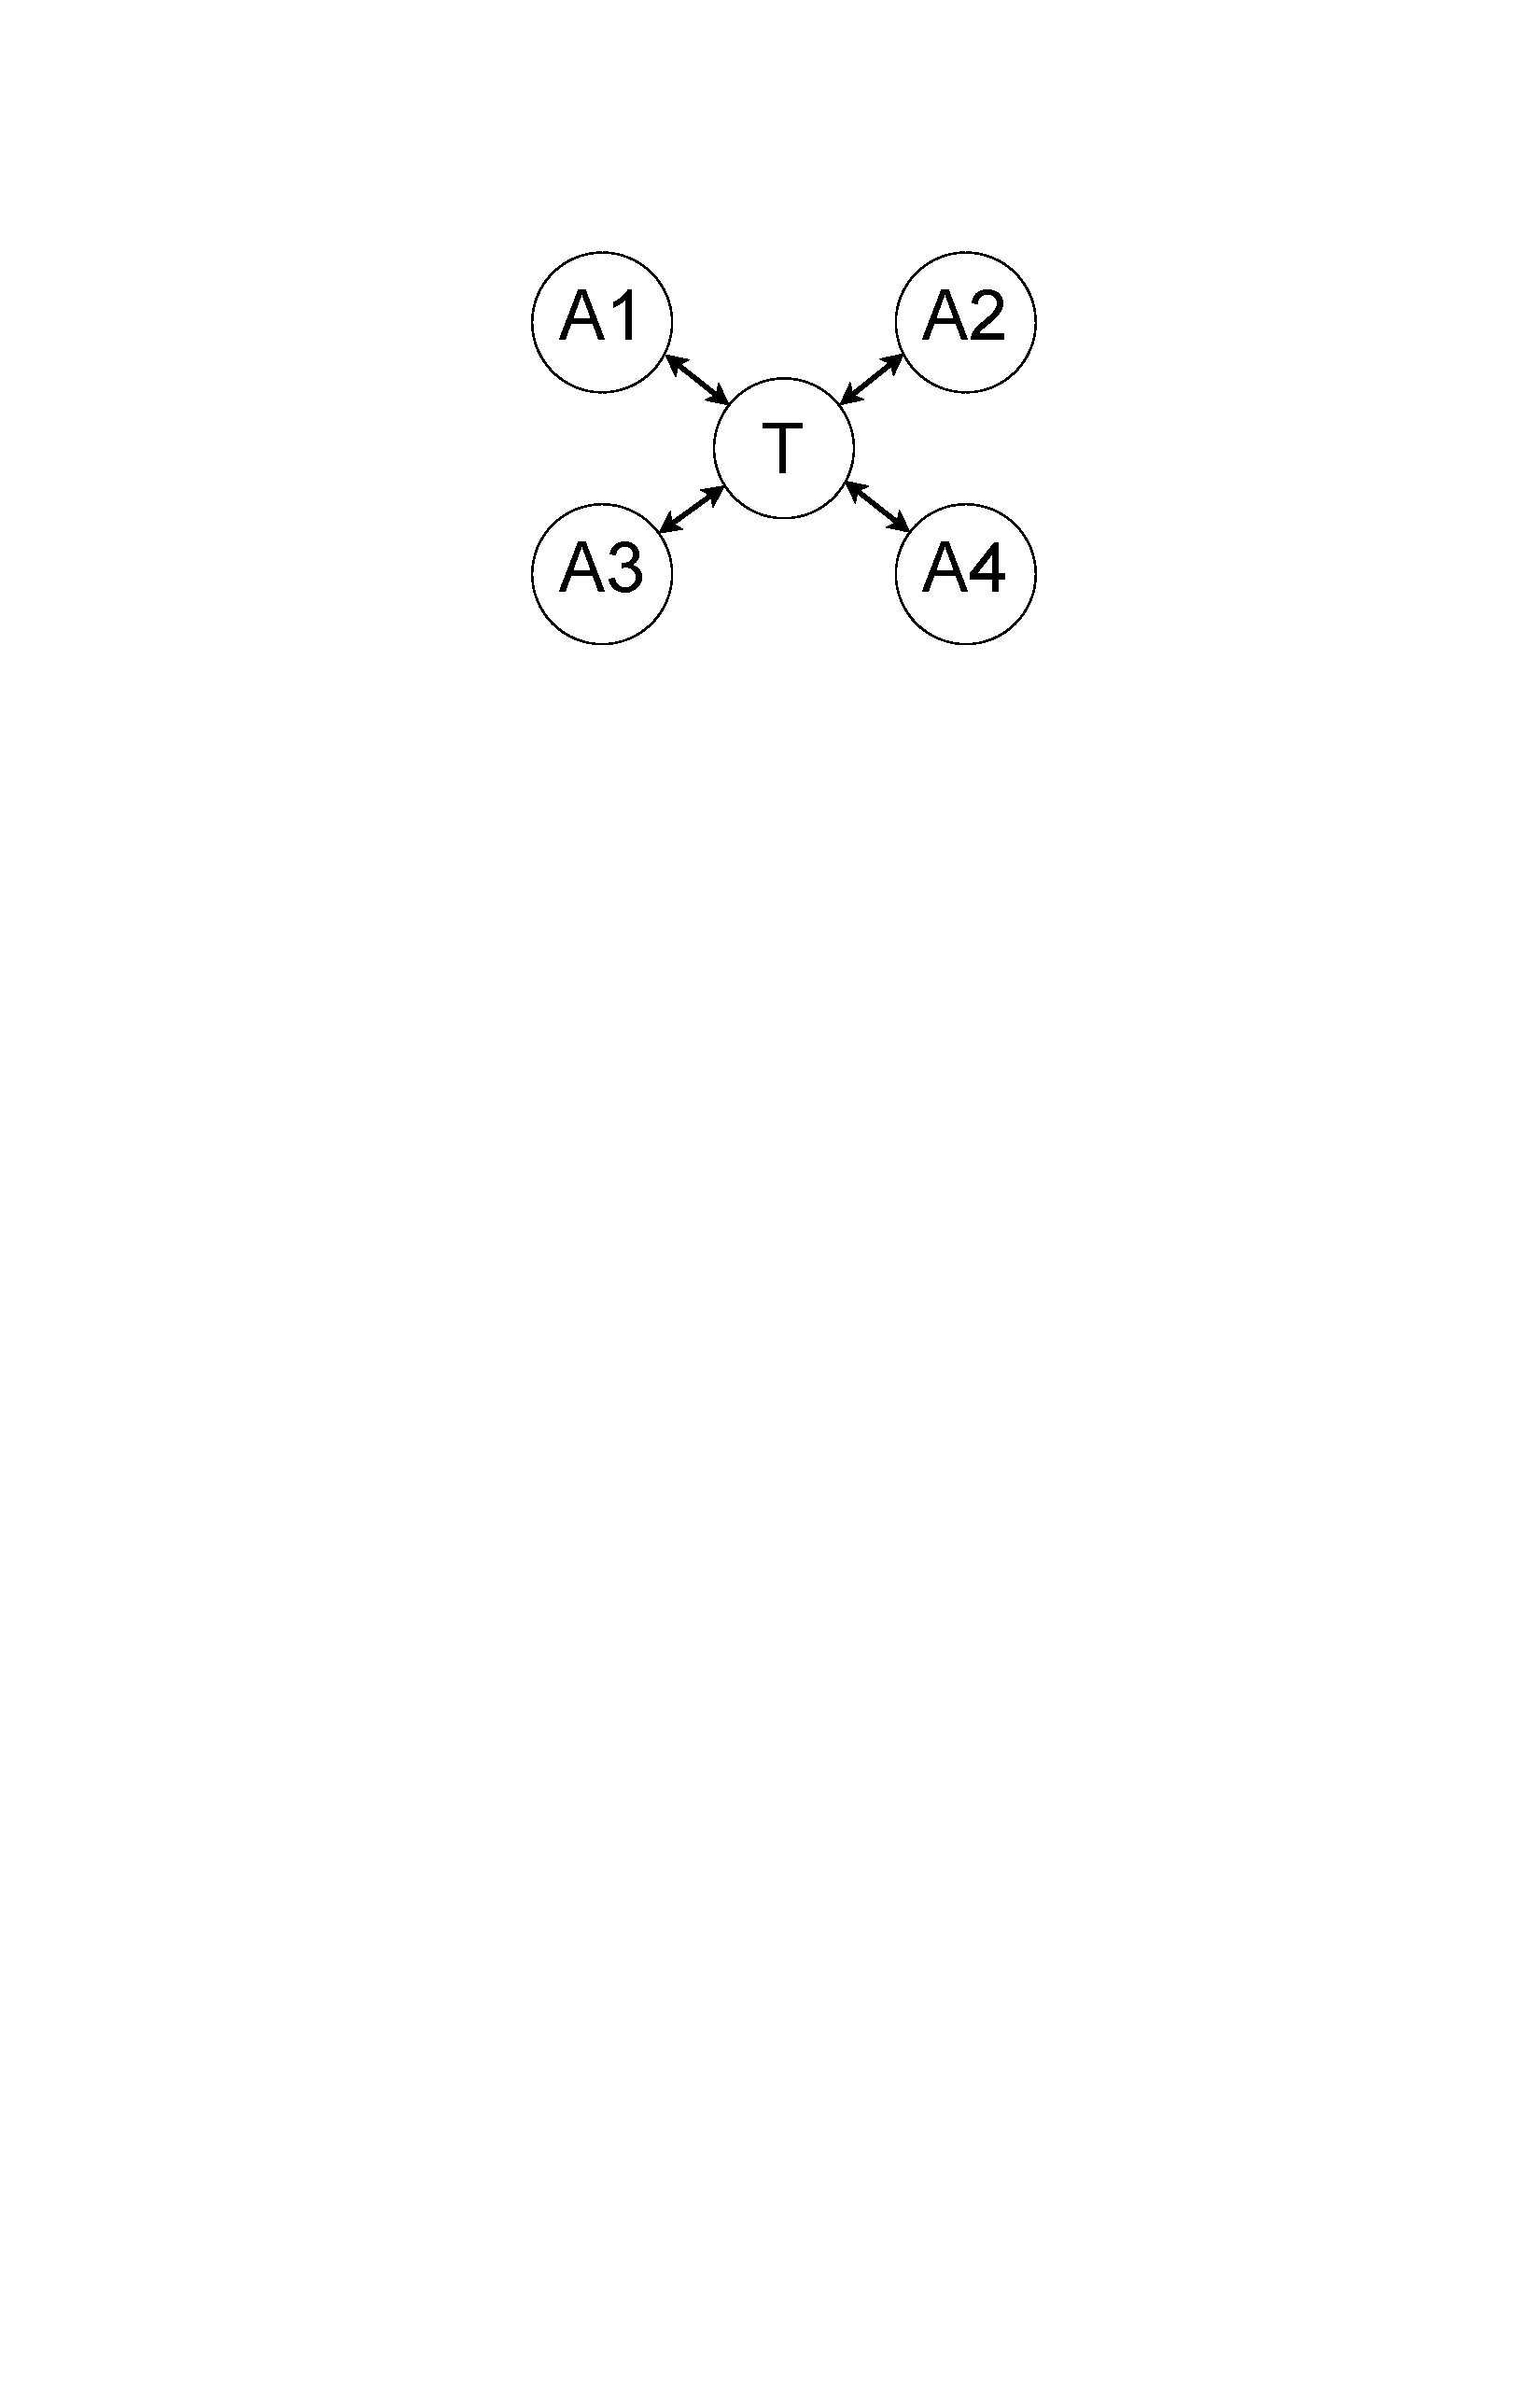
\includegraphics[width=1\linewidth]{pic2.pdf}
	\caption{Сеть с выделенным доверенным центром.}
	\label{p3}
	\end{minipage}
	\end{center}
\end{figure}

Протокол распространения ключей должен реализовывать следующие цели:
\begin{itemize}
    \item аутентификация сторон протокола;
    \item защита от повтора;
    \item аутентификация ключа;
    \item подтверждение владения ключом;
    \item совершенная секретность;
    \item формирование новых ключей;
    \item ограниченная защита от атак и/или отказа в обсуживании.
\end{itemize}

Этап работы протокола с доверенным центром:
\begin{enumerate}
    \item Доверенный центр создает секрет, известный только ему. Секрет из себя представляет пару из закрытого и открытого ключей.
    \item Для каждого нового участника сети доверенный центр, используя секрет, создает сертификат, который позволяет новому участнику 
    вырабатывать сеансовые ключи с другими участниками.
    \item Здесь начинается общение участников. Они предъявляют друг другу идентификаторы, которые получили от доверенного центра. Далее используя эту информацию они могут сгенерировать секретный сеансовый ключ для общения мужду собой.
\end{enumerate}

Изучим более подробно схемы распределения ключей с доверенным центром на примере протокола Жиро. 
\section{Протокол Girault}

\textbf{Протокол Жиро} представляет из себя криптографический протокол, благодаря которому две стороны могут получить общий секретный ключ, не используя при этом явную сертификацию. 
Данный протокол использует полученный ключ для шифрования сообщений с помощью симметричного шифрования.

Схема Жиро решает проблему протоколов, основанных на подтверждении личности. Например, в схемах Шамира используются 2 атрибута - открытый ключ $I$ и закрытый ключ $s$. Так как закрытый ключ $s$ определяется непосредственно участником протокола, то он может начать выдавать себя за другого пользователя в любой момент.
Также при возникновении противоречивых свидетельств у пользователя и подтверждающей стороны - невозможно определить, кто из них злоумышленник.

Жиро смог решить эту проблему, изменив процесс сертификации - ключи сами себя сертифицируют. В схеме Жиро присутствует доверенный центр,  благодаря которому обмен информацией 
между пользователями надежно защищён. Теперь только доверенный центр может генерировать скрытую сертификацию для этих ключей. 
Надёжность схемы Жиро строится на стойкости криптосистемы RSA.
\\
Первостепенно участники протокола проходят аутентификацию перед доверенный центром $T$, а также получают открытый ключ:
\begin{enumerate}
    \item Начальный этап: доверенный центр Т 
    \begin{enumerate}
        \item выбирает общий модуль $n = p \cdot q$, где $p$ и $q$ - большие простые числа;
        \item далее выбирает пару из закрытого $K_{T, priv} = (d,n)$ и открытого $K_{T, pub}=(e,n)$ ключей; 
        \item выбирает элемент $g$ поля $Z_n^\times$ максимального порядка;
        \item публикует в открытом доступе для участников параметры: $n, \; e, \; g$.
    \end{enumerate}
    \item Основной этап: участники 
    \begin{enumerate}
        \item выбирают себе закрытый ключ $s_i$ (каждый свой) и идентификатор $I_i$;
        \item вычисляют $v_i = g ^{-s_i} mod n$;
        \item отправляют $v_i$ доверенному центру;
        \item используя протокол аутентификации сторон участники доказывают доверенному центу $T$, что владеют закрытым ключом, не раскрывая его значение;
        \item далее получают от доверенного центра свой открытый ключ: $P_i = (v_i - I_i)^d = (g^{-s_i} -I_i)^d mod \; n$.
    \end{enumerate}
    \item В результате для каждого участника будет выполняться: $P_i^e+I_i = g^{-s_i} mod \; n$.
\end{enumerate}
Далее рассмотрим аутентификацию конечных участников. Пусть есть две стороны обычно их называют Alice и Bob, тогда процесс аутентификации между ними выглядит так:
    \begin{enumerate}
        \item Alice выбирает случайное $R_A$  и передает Bob; 
        $$A \rightarrow \{I_A, P_A, t = g^{R_A} \; mod \; n\} \rightarrow B $$
        \item Bob также выбирает случайное $R_B$;
        $$B \rightarrow \{R_B\} \rightarrow A $$
        \item Alice вычисляет значение $y$, которое смогла посчитать благодаря $R_B$; $$A \rightarrow \{y = R_A + s_A \cdot R_B \; mod \; n\} \rightarrow B $$
        \item Bob вычисляет $v_A = P_A^e + I_A \; mod \; n  = g^{-s_A} \; mod \; n $;
        \item Bob проверяет, что $t = g^y\cdot v_A^{R_B} = g^{R_A+s_a \cdot R_B}\cdot (g^{-s_A})^{R_B} = g^{R_A}  \; mod \; n$;
    \end{enumerate}

    Данные протокол построен на том, чтобы участник коммуникаций смог доказать, что он знает закрытый ключ, но при этом не сообщал значение этого ключа. При выполнении данного протокола вероятность того, что Bob примет сообщения Alice составляет практически 100\% (стоит учитывать возможные помехи сети).
    В случае, если появится мошенник, который постарается выдать себя за участника протокола,то этот негодяй будет раскрыт с вероятностью $1 - 2^{-30}$. \\
    А теперь рассмотрим поподробнее схему Жиро, в рамках которой генерируется общий секретный ключ и происходит обмен данными. По сути это, что происходит в пунктах 3 - 4 аутентификации.
\subsection{Схема Жиро}
\textbf{Схема Жиро} состоит из нескольких этапов обмена открытой информацией и вычисления ключа. Ниже опишем алгоритм протокола:
\begin{enumerate}
    \item Alice посылает свой открытый ключ и идентификатор; $$Alice \; \rightarrow \{ P_A, I_A\} \rightarrow Bob$$
    \item Bob вычисляет $K$: $$K = (P_A^e + I_A)^{s_B} \; mod \; n$$
    \item Bob высылает свои параметры: $$ Bob \; \rightarrow \{ P_B, I_B\} \rightarrow Alice $$
    \item Alice вычисляет $K$: $$K =(P_B^e + I_B)^{s_A} \; mod \; n$$.
\end{enumerate}
В результате работы схемы стороны сгенерировали одинаковый общий сеансовый ключ.
$$K_{AB} = (P_A^e + I_A)^{s_B} = (g^{-s_A})^{s_B} = g^{-s_As_B} \; mod \; n ;$$
$$K_{BA} = (P_B^e + I_B)^{s_A} = (g^{-s_B})^{s_A} = g^{-s_As_B} \; mod \; n ;$$
$$K = K_{AB} =K_{BA} \; mod \; n ;$$

Данная схема помимо генерации ключей обеспечивает также аутентификацию ключа - только легальные пользователи могут вычислить корректное значение общего сессионного ключа.
А полученный ключ используется для шифрования дальнейшего обмена данными с помощью алгоритмов симметричного шифрования.

\section{Криптографическая стойкость}
Разберемся к каким атакам у данного протокола есть стойкость.
\subsection{Защита от атаки подменой}
\textit{Атака подменой - злоумышленник с помощью легально переданного соообщения составляет новое и передает его в следующем раунде протокола под видом другого сообщения}.
\\
\par 
Если ключи само сертифицированные, то нельзя проверить подлиность значений $(I_A, P_A, s_A)$, так как они не подтверждены доверенным центром $T$.\\
Рассмотрим следующую ситуацию: появляется 3ий участник - Carol, который возьмет идентификатор Alice $I_A$ и поддельный ключ $s_A'$, тогда он может вычислить значение $v_A = P_A^e + I_A = g^{-s_A} \; mod \; n$  и пройти аутентификацию перед $T$. Но вычислить $s_A$, зная $v_A$ -  это задачка дискретного логарифмирования, которая является неразрешимой.
А без $s_A$ Carol не сможет сформировать ключ $K$ и соответственно продолжить притворяться Alice. Значит, протокол Жиро защищен от атаки подменой.
\subsection{Защита от атаки повтором}

\textit{Атака повтором - злоумышленник записывает все сообщения, проходящие в одном сеансе протокола, а далее повторяет их в новом, выдавая себя за одного из участников первого сеанса.}
\\
\par Пусть Carol перехватил сообщение Alice $(I_A, v_A, s_A)$ и через некоторе время решает отправить его доверенному центру $T$. 
Проверив параметры, $T$ поймет, что сообщение передано повторно, так как $I_A$ уже использовался, и завершит сеанс. Таким образом, протокол Жиро защищен от атаки повтором.
\section{Литература}

\begin{thebibliography}{}
    \bibitem{litlink1}  Брюс Шнайер -  \href{https://lib.mipt.ru/book/n/00013022000cdbe8096da0a688d3a130/Shnaier-B-Prikladnaya-kriptografiya-Protokoly-algoritmy-i-ishodnye-teksty-na-yazyke-S.pdf}{"Прикладная криптография. Протоколы, алгоритмы и исходные тексты на языке С."}
    \bibitem{litlink2}  Венбо Мао -  \href{https://lib.mipt.ru/book/266371/?q=+криптографические+протоколы}{"Современная криптография. Теория и практика."}
    \bibitem{litlink1}  Википедия -  \href{https://ru.wikipedia.org/wiki/Протокол_Жиро}{"Протокол Жиро."}
    \bibitem{litlink1}  M. Girault -  \href{https://doi.org/10.1007/3-540-46416-6_42}{"Self-Certified Public Keys. С. 490—497."}
\end{thebibliography}
\end{document}

